\subsection{Pruebas de la versión: 2} \label{chp:pruebasV2}
En esta sección se describen los resultadods de las pruebas realizadas de la segunda versión del algoritmo de optimización de horarios.\\

Como consideración tenemos que las pruebas fueron realizadas en una laptop dell Inspiron 15 con procesador intel i5 5ta generación 4gb de memoria ram usando el sistema operativo debian 9.\\


\subsubsection{Pruebas realizadas}

Inicialmente las funciones que comprenden el algoritmo fueron probadas por separado. \\

\begin{itemize}
	\item Se corroboró que la función de generar Población utilizara todas las opciones de Materia-Profesor disponibles y que el resultado tuviera la estructura que hemos definido. 
	
	\item Se probó la función de evaluación, para corroborar que las restricciones ingresadas sean tomadas en cuenta al momento de asignar una calificación a un horario.
	
	\item Se probaron las funciones de mutación de forma que el resultado arrojado después de llevar a cabo dichos operadores sea en realidad distinto a la entrada del mismo así como se corroboró que se llevaran a cabo de la manera esperada.
	
\end{itemize}

Una vez que se corrigieron los errores arrojados por las pruebas de de la primera versión del algoritmo se utilizó el mismo esquema de pruebas. Para corroborar que el funcionamiento fuera correcto, utilizamos la estructura educativa actual de la ESCOM para el nivel 2 y el turno matutino. Utilizando estos datos, se creó una población inicial aleatdforia, una población inicial usando la función generar Población y se tomó como ejemplo la estructura tal cual se utiliza hoy en día.\\

Haciendo uso de la función de evaluación determinamos que la calificacion de la población aleatoria fue de 1315, la calificación de la población generada por la función generar Población fue de 20 y finalmente la calificación de la estructura de ejemplo fue de 36. Teniendo en cuenta que nuestro problema es de minimización y la calificación óptima es 0, el horario generado por la función de población inicial fue el mejor adaptado sin llegar a ser el óptimo.\\

Una vez que se operaron las funciones de mutación sobre la población generada por nuestra función de generar Población, se logró disminuir la calificación hasta llegar a 0 indicando así que nuestro algoritmo arroja soluciones óptimas de acuerdo a las restricciones planteadas.\\

Finalmente se determinó utilizar dos criterios de paro, si bien alcanzar una calificación óptima funciona como uno, la complejidad del problema implica una alta probabilidad de no encontrar soluciones óptimas en todas las ocasiones que se ejecute el algoritmo. Por lo tanto un criterio de paro alternativo debe ser un número determinado de iteraciones, el cúal se determinó de forma experimental de la siguiente manera.\\

En cinco ocasiones se tomó la calificación arrojada por la función de evaluación para el resultado después de llevar a cabo la mutación un número determinado de veces el cúal fue disminuyendo hasta llegar al 0 en cada uno de las 5 corridas. En la figura \ref{fig:PruebaV2} se muestran los resultados del experimento y en la figura \ref{fig:grafV1} se muestra la gráfica de los mismos donde se puede apreciar que a partir de las 20,000 iteraciones se alcanza la solución óptima en cada ocasión que se ejecuta el procedimiento, por lo tanto se define como criterio alternativo de paro alcanzar dicho número de iteraciones.\\
 
 \begin{figure}[htbp!]
 	\begin{center}
 		\fbox{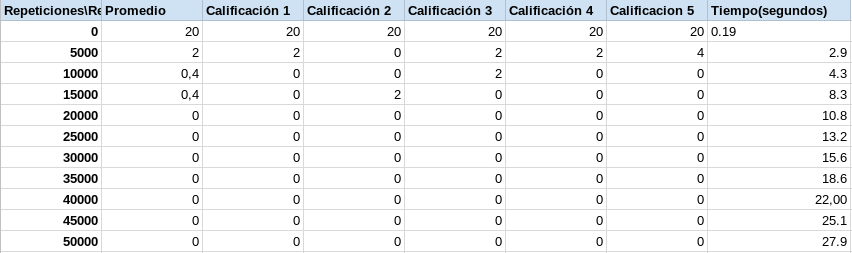
\includegraphics[width=.7\textwidth]{ModeloComportamiento/Algoritmo/imagenes/tabla2.png}}
 		\caption{Determinación experimental del criterio de paro}
 		\label{fig:PruebaV2}
 	\end{center}
 \end{figure}


\begin{figure}[htbp!]
	\begin{center}
	\fbox{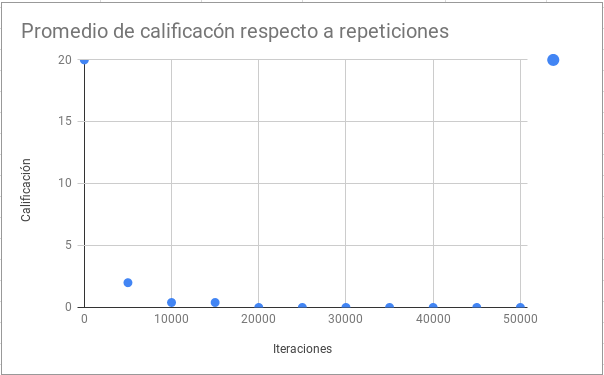
\includegraphics[width=.7\textwidth]{ModeloComportamiento/Algoritmo/imagenes/grafica2.png}}
		\caption{Gráfica de mejora}
		\label{fig:grafV2}
	\end{center}
\end{figure}

